这一节中,我们首先回顾 Attention 机制中的基本概念(\ref{subsec:attention})。接下来,我们将介绍后续各类算法中用到的背景知识,包括线性化自注意力(\ref{sec:linearattn})指数移动平均(\ref{subsec:ema})。


\subs{Attention 机制}
\label{subsec:attention}
我们使用 $\boldsymbol{X} = \{\mathbf{x}_1, \mathbf{x}_2, \ldots, \mathbf{x}_n\} \in \mathbb{R}^{n\times d}$ 表示具有长度 $n$ 的输入表示序列。
其中 $\mathbf{x}_t \in \mathbb{R}^{d}$ 是 $\boldsymbol{X}$ 中第 $t$ 个标记的 $d$ 维表示向量,其中 $t \in \{1, 2, \ldots, n\}$。
令 $\boldsymbol{Y} =\{\mathbf{y}_1, \mathbf{y}_2, \ldots, \mathbf{y}_n\} \in \mathbb{R}^{n\times d}$ 为每一层的输出表示序列,其与输入 $\boldsymbol{X}$ 具有相同的长度 $n$。
%序列模型的目标是计算 $\boldsymbol{Y}$,以捕获从 $\boldsymbol{X}$ 中解决目标任务所需的上下文信息。
在本文中,我们假设输入和输出序列的表示具有相同的维度 $d$。
\subsubs{注意力和多头注意力}
\label{subsubsec:attention}
注意力机制是一种长序列的建模手段,其可以表示为查询 $\boldsymbol{Q}\in \mathbb{R}^{n\times d} $,键 $\boldsymbol{K}\in \mathbb{R}^{n\times d}$ 和值 $\boldsymbol{V}\in \mathbb{R}^{n\times d}$ 的函数。

\begin{equation}
    \label{eq:attention}
    \mathrm{Attention}(\boldsymbol{Q}, \boldsymbol{K}, \boldsymbol{V})=f\left( \frac{\boldsymbol{Q} \boldsymbol{K}^T}{\tau} \right) \boldsymbol{V}
\end{equation}

其中,$f(\cdot)$ 是一个注意力函数,例如 softmax 函数 $f_{\mathrm{softmax}}(\cdot)$~\cite{bahdanau2015neural} 或最近提出的平方 ReLU 函数 $f_{\mathrm{relu^2}}(\cdot)$~\cite{hua2022transformer}。
$\tau$ 是一个温度因子,通常设置为 $\tau = \sqrt{d}$(对于 $f_{\mathrm{softmax}}(\cdot)$)或 $\tau = n$(对于 $f_{\mathrm{relu^2}}(\cdot)$)。Attention 函数要求 $\boldsymbol{K}$ 和 $\boldsymbol{V}$ 具有相同的序列长度。直观上,Attention 是对值 $\boldsymbol{V}$ 在整个时序上进行线性组合,而组合系数则是由相应位置上 $\boldsymbol{Q}$ 和 $\boldsymbol{K}$ 的关系决定。

为了更好地在建模序列中的复杂关系,我们可以将输入投影到多个不同的表征空间,在这些空间中分别进行注意力操作,之后再将结果连接并投影到一个完整的空间中。这就多头自注意力机制(Multi-head Attention)
\begin{equation}
\mathrm{MHA}(\boldsymbol{Q}, \boldsymbol{K}, \boldsymbol{V}) =\mathrm{Concat}\left(\mathrm{head}_1, \ldots, \mathrm{head}_{\mathrm{h}}\right) W^O \\
\end{equation}
MHA 表示 Multi-head Attention,而 $\mathrm{head}_i$由
\begin{equation}
    {\mathrm{head}_{\mathrm{i}}}  =\mathrm { Attention }\left(\boldsymbol Q W_{qi}, \boldsymbol K W_{ki}, \boldsymbol V W_{vi}\right)
\end{equation}
给出。其中 $W_{qi}, \ W_{ki}, \ W_{vi}$ 为各个注意力头所使用的投影矩阵。由于投影到的子空间不同,各个注意力头可以产生不同的组合系数,进而提取序列中更复杂的关系。

\subsubs{自注意力}
\label{subsubsec:self-attention}
传统的自注意力机制是一个对已有序列的变换函数 $\mathrm{SelfAttention}: \mathbb{R}^{n\times d} \rightarrow \mathbb{R}^{n\times d}$,用于提取序列中的时序关联信息。其就是将多头注意力中的 $\boldsymbol{Q}, \ \boldsymbol{K}, \ \boldsymbol{V}$ 都设为输入的序列 $\boldsymbol{X}$,即可表示为
\begin{equation}\label{eq:self-attention}
\mathrm{SelfAttention}(\boldsymbol{X}) = \mathrm{MHA}(\boldsymbol{X}, \boldsymbol{X}, \boldsymbol{X})
\end{equation}

\subsubs{复杂度分析}
\label{subsubsec:attn-complexity}

从 Attention 的定义式 ~\ref{eq:attention} 中,我们可以定义注意力矩阵 $\boldsymbol{A}=f(\frac{\boldsymbol{Q}{\boldsymbol{K}}^{T}}{\tau(\boldsymbol{X})})\in \mathbb{R}^{n\times n}$,其表示了 $\boldsymbol{X}$ 中每对标记之间的依赖强度。注意力矩阵提供了一种灵活而强大的机制,可以直接表征输入序列中任意距离两元素间的关联程度。然而,使用 $h$ 个注意力头计算 $\boldsymbol{A}$ 需要 $O(n^2)$ 的时间和空间,这种平方级的开销成为限制 Attention 长序列处理能力的重要瓶颈。


\subs{自注意力的线性化}
\label{sec:linearattn}
我们首先考虑注意力函数的输出
\begin{equation}
   \mathcal{O} = \mathcal{A}(x) = \left[\mathcal{O}_1,\hdots, \mathcal{O}_N \right]^T, \quad \mathcal{O}_i
 = \sum_j \frac{\mathcal{S}(Q_i,K_j)}{\sum_j \mathcal{S}(Q_i,K_j)}V_j,
    \label{eq: generalized att}
\end{equation}
我们可以选择任何相似性函数来计算注意力矩阵。为了保持线性计算预算,一种解决方案是采用可分解的相似性函数,使得:
\begin{equation}
\textstyle{
\mathcal{S}(Q_i, K_j) = \phi(Q_i)\phi(K_j)^T,
\label{eq: decompose}
}\end{equation}
其中$\phi$是一个核函数,将查询和键映射到它们的隐藏表示中。然后,我们可以将公式~\ref{eq: generalized att} 重写为核函数的形式:
\begin{equation}
\textstyle{
O_i = \frac{\sum^{N}{j=1}(\phi (Q_i) \phi({K_j})^T) V_j}{\sum^{N}{j=1}(\phi (Q_i) \phi({K_j})^T)},
\label{eq: rewrite att}
}\end{equation}
通过矩阵乘积的特性,实现线性复杂度下的注意力操作:
\begin{equation}
\textstyle{
(\phi (Q) \phi({K})^T) V = \phi (Q) (\phi({K})^T V),
\label{eq: linear form}
}\end{equation}
在式\eqref{eq: linear form}中,我们首先计算 $\phi({K})^T V \in\mathbb{R}^{d \times d}$,然后再乘以 $\phi(Q)\in\mathbb{R}^{N \times d}$。通过使用这个技巧,我们只需要 $O(Nd^2)$ 的计算复杂度。
需要注意的是,在典型的自然语言任务中,一个头部的特征维度 $d$ 通常远小于输入序列的长度 $N$($d\ll N$),因此我们可以安全地忽略 $d$,从而实现 $O(N)$ 的计算复杂度,如图\ref{fig: linear} 所示。

\begin{figure}[t]
\begin{center}
{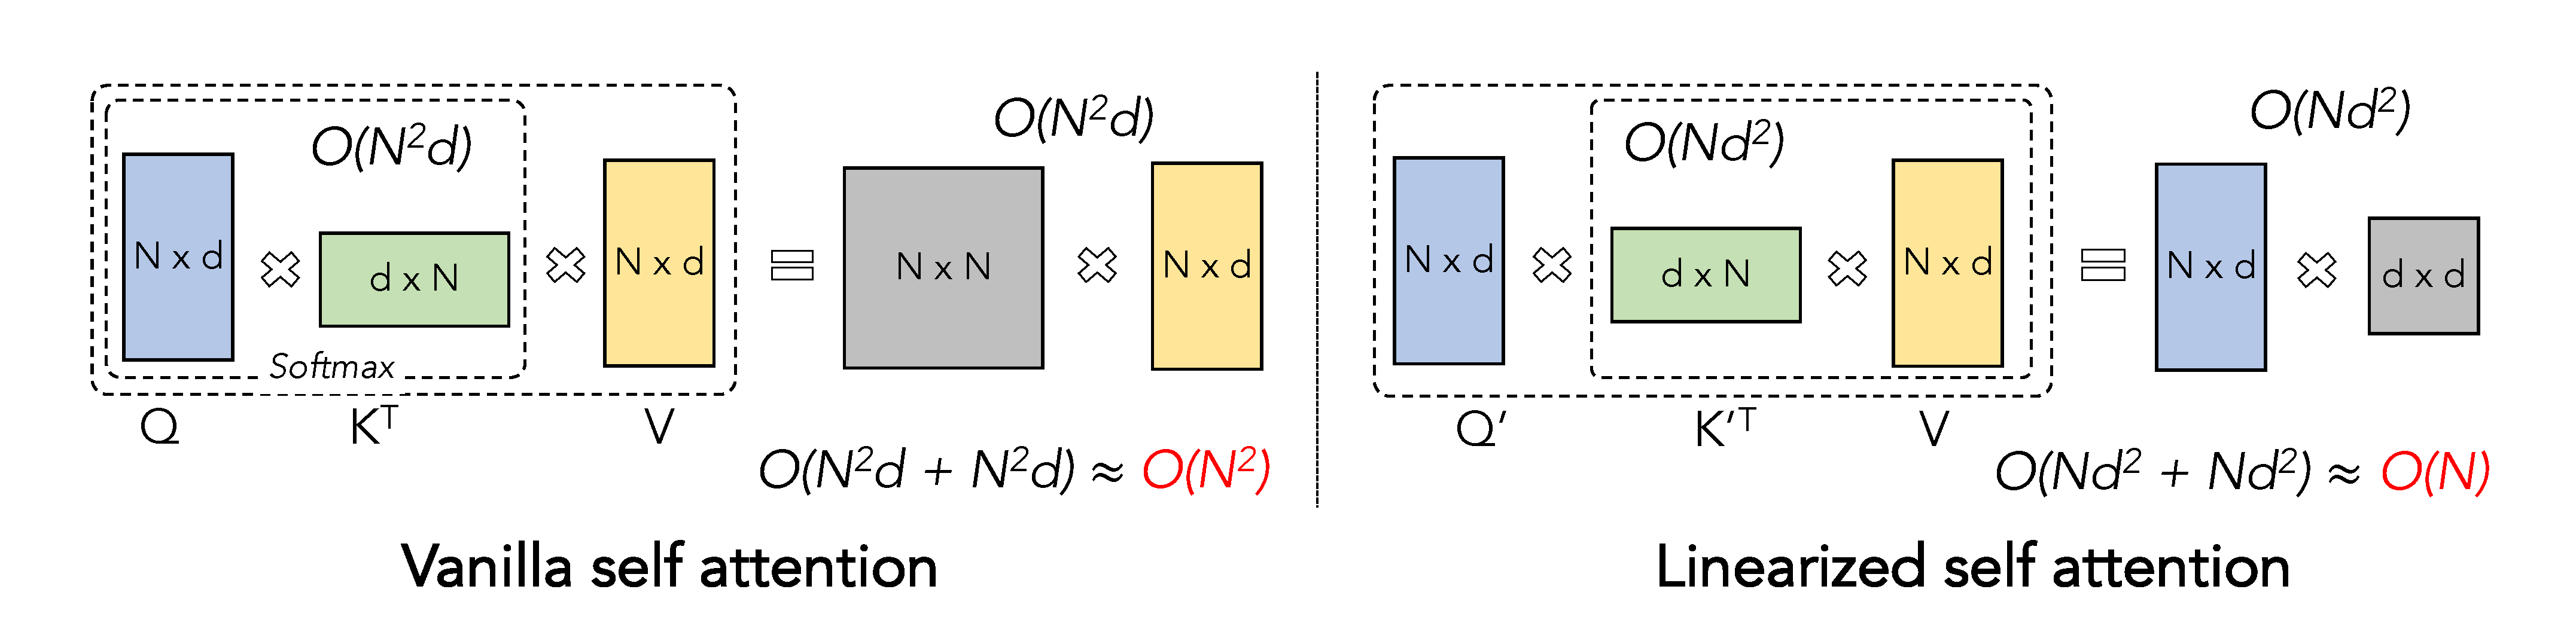
\includegraphics[width=1\linewidth]{figs/cosformer/linear3.pdf}}
\vspace{-10mm}
\end{center}
\caption{基于原始自注意力机制的计算过程(左)和线性化注意力机制的计算过程(右)。输入长度为 $N$,特征维度为 $d$,其中 $d\ll N$。同一框中的张量相关联用于计算。线性化的公式实现了 $O(N)$ 的时间和空间复杂度。摘自~\cite{zhen2022cosformer}}
\vspace{-4mm}
\label{fig: linear}
\end{figure}
\vspace{-2mm}


\subs{指数移动平均(EMA)}
\label{subsec:ema}
移动平均是一种经典的序列数据建模方法,在时间序列数据中广泛用于平滑短期波动并突出长期趋势或周期。指数移动平均(EMA)是移动平均的一种特殊情况,它应用了指数衰减的加权因子。
沿用 ~\ref{subsec:attention} 中对输入输出序列的符号,EMA 可以递归地表示为 $\boldsymbol{Y}$:
\begin{equation}
\label{eq:ema}
\mathbf{y}_t = \boldsymbol{\alpha} \odot \mathbf{x}_t + (1 - \boldsymbol{\alpha}) \odot \mathbf{y}_{t-1},
\end{equation}
其中 $\boldsymbol{\alpha} \in (0, 1)^{d}$ 是 EMA 系数,表示权重减小的程度,$\odot$ 是逐元素乘积。
较高的 $\boldsymbol{\alpha}$ 会更快地衰减旧观测值的权重。EMA偏好于局部依赖关系,并限制了远距离依赖关系。尽管在 \eqref{eq:ema} 中采用了循环形式,EMA 的计算事实上可以表示为 $n$ 个独立的卷积操作,可以使用快速傅里叶变换(FFT)高效计算~\cite{ma2023mega}。

在 \ref{subsec:mega} 中,我们将介绍一种将 EMA 嵌入注意力计算中的计算方式 MEGA,并进一步给出具有线性时间复杂度近似算法 MEGA-chunk(\ref{subsec:mega-chunk})。